%------------------------------------------------
\section{Введение}
%------------------------------------------------
\begin{frame}
 \frametitle{Актуальность}
 	\begin{itemize}
 		\item Исследование кварк-глюонной плазмы;
 		\item Разрешение проблемы "спинового кризиса";
 		\item Изучение Электрического Дипольного Момента;
 		\item Поиск аксионоподобных частиц.
 	\end{itemize}

	 %\begin{figure}
	 %	\centering
	 %	\includegraphics[width=0.24\linewidth]{"images/EDM CP"}
	 %	\includegraphics[width=0.74\linewidth]{"images/EDM World"}
	 %\end{figure}

\end{frame}
%------------------------------------------------
\begin{frame}
	\frametitle{Цель и Задачи исследования}
	\textbf{Целью} данной диссертации является изучение особенностей поведения лёгких поляризованных пучков в предлагаемой дуальной структуре, а также исследования ЭДМ с использованием квази-замороженной концепции.\newline \newline
	Для достижения поставленной цели необходимо было решить следующие \textbf{задачи}:
	\begin{itemize}
		\item Расчёт времени внутрипучкового рассеяния и стохастического охлаждения;
		\item Моделирование магнитооптики с модулированной дисперсионной функцией;
		\item Проведение численного моделирования продольной динамики частиц;
		\item Изучение «квази-замороженного» спина для измерения ЭДМ дейтрона и протона;
	\end{itemize}
\end{frame}
%------------------------------------------------
\begin{frame}
	\frametitle{Научная новизна}
	\begin{itemize}
		\item	Впервые предложена дуальная структура для тяжелых ионов и легких частиц для коллайдера NICA;
		\vspace{1em}
		\item 	Впервые предложены методы подавления дисперсии поворотной аркой в резонансной магнитооптической структуре с отсутствующими магнитами;
		\vspace{1em}
		\item	Впервые исследован метод скачка критической энергии с использованием барьерного ускоряющего потенциала с учётом ограничений по продольной микроволновой неустойчивости;
	\end{itemize}
	
\end{frame}
%------------------------------------------------
\begin{frame}
	\frametitle{Научная новизна}
	\begin{itemize}
		\item 	Были проведены исследования продольной динамики с учётом высших порядков разложения по импульсу, а также влиянием импеданса. На их базе сформулированы ограничения на величину и темп скачка критической энергии;
		\vspace{1em}
		\item	Были разработаны 8- и 16-периодичная квази-замороженная структура Nuclotron для выделения ЭДМ сигнала лёгких ядер;
		\vspace{1em}
		\item	Была разработана структура коллайдера NICA с обводными каналами, неориентированная изначально на эксперименты по поиску ЭДМ дейтрона методом квази-замороженного спина;
	\end{itemize}
\end{frame}
%------------------------------------------------
\begin{frame}
	\frametitle{Практическая значимость}
	Исследования направлены на формирование полноценной физической программы в комплексе Nuclotron-NICA. \\
	Применение изложенных в работе подходов возможно и на других похожих установках без потери общности.
\end{frame}
%------------------------------------------------
\begin{frame}
	\frametitle{Объект исследования}
	% TODO: \usepackage{graphicx} required
	\begin{figure}
		\centering
		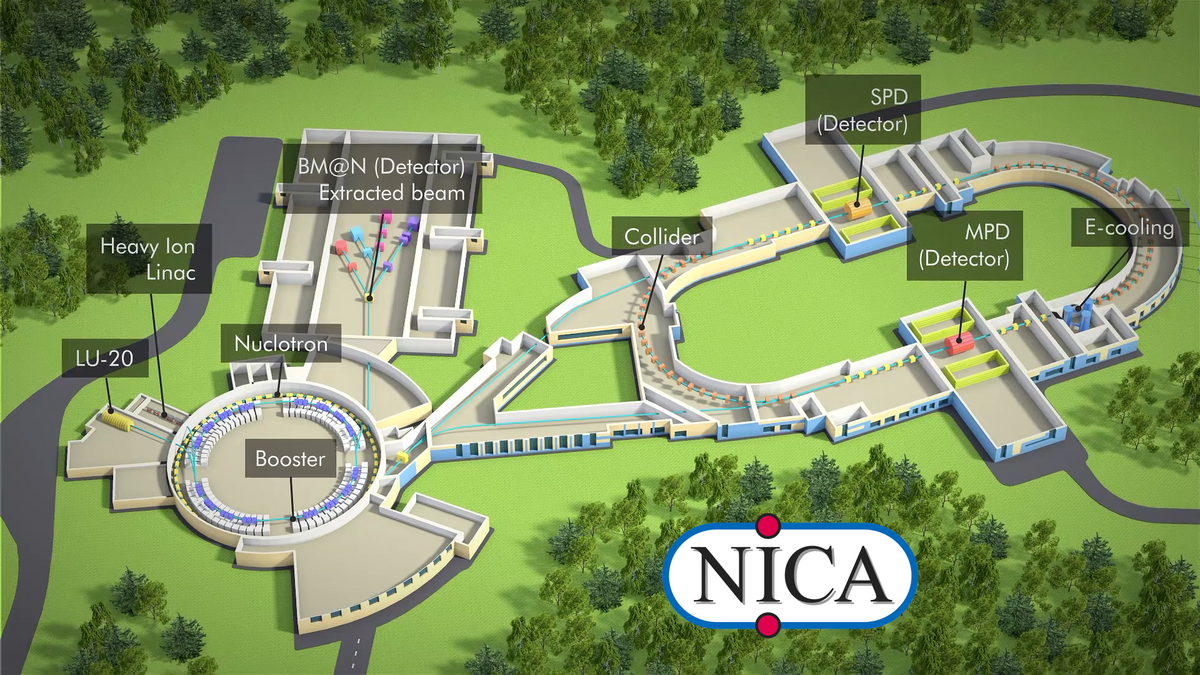
\includegraphics[width=0.6\linewidth]{images/NICA}
	\end{figure}
	В работе отдается приоритет исследованиям свойств пучков частиц, где ускоритель выступает в роли детектирующего устройства.
\end{frame}
%------------------------------------------------
\begin{frame}
	\frametitle{Методы исследования}
	\begin{enumerate}
		\item	Аналитические и численные;
		\item	Экспериментальные;
	\end{enumerate}
	\vspace{2em}
	\textbf{Математическое и компьютерное моделирование}. Были использованы программы для расчёта поперечной динамики: MAD-X, OPTIM, BMAD, продольной динамики: BLonD; спин-орбитальной динамики: COSY Infinity.\\
	\vspace{1em}
	\textbf{Экспериментальные} методы исследования заключаются в изучении динамики пучка с применением скачка критической энергии и без него.
	Соискатель лично участвовал в сеансе на синхротроне У-70 в г. Протвино, Россия в 2023 году.

\end{frame}
%------------------------------------------------
\begin{frame}
	\frametitle{Основные положения, выносимые на защиту}
	\begin{itemize}
		\item 	Предложена реализация дуальной структуры для комплекса NICA-Nuclotron, оптимальная для тяжелых ионов с точки зрения ВПР и лёгких частиц с поднятой критической энергией;
		\vspace{1em}
		\item	Реализован метод вариации критической энергии для коллайдера NICA с отсутствующими магнитами при подавлении дисперсионной функции двумя семействами квадруполей и двумя крайними ячейками;
		\vspace{1em}
		\item	Представлены результаты моделирования продольной динамики с учётом высших порядков разброса по импульсам и моделей продольных импедансов в окрестности критической энергии и сравнение с экспериментальными данными на У-70;
	\end{itemize}
\end{frame}
%------------------------------------------------
\begin{frame}
	\frametitle{Основные положения, выносимые на защиту}
	\begin{itemize}
		\item	Проведен анализ использования гармонического ВЧ при процедуре скачка в коллайдере NICA. Для барьерного ВЧ представлены данные моделирования продольной динамики. Предложено сокращение длины между барьерами из-за продольной микроволновой неустойчивости;
		\vspace{1em}
		\item	Предложены модернизированные 8/16-периодичные структуры Nuclotron с квази-замороженным спином для исследования ЭДМ лёгких ядер, с сохранением функции бустера;
		\vspace{1em}
		\item	Применен метод фильтров Вина для сохранении направления поляризации на основе введения обводных каналов в структуре коллайдера NICA с квази-замороженным спином;
	\end{itemize}
\end{frame}
%------------------------------------------------